\pdfsuppresswarningpagegroup=1

\documentclass[
    %handout,
]{beamer}

\usetheme{Boadilla}
\usecolortheme{seahorse}
\usepackage{pifont}
\usepackage{pgfplots}
\usepackage{svg}
\usepackage{t1enc}
\usepackage{bbding}
\usepackage{fontawesome5}
\usepackage{minted}
\usepackage[hungarian]{babel}
\usepackage[none]{hyphenat}

\pgfplotsset{
    tick label style = {font = {\fontsize{8 pt}{14 pt}\selectfont}},
    every axis label = {font = {\fontsize{8 pt}{14 pt}\selectfont}},
    label style = {font = {\fontsize{10 pt}{20pt}\selectfont}},
    legend style = {font = {\fontsize{6 pt}{10 pt}\selectfont}},
}

\titlegraphic{
\includegraphics[width=2cm]{elte_cimer_szines}}
\title[HoloDB]{HoloDB: szintetikus adatok on-the-fly szolgáltatása relációs adatbázisként}
\author[Horváth Dávid]{Horváth Dávid \\ ~ \\ { \footnotesize Témavezető: Dr. Vincellér Zoltán, Mesteroktató }}
\institute[ELTE-IK]{ELTE Informatikai Kar, Információs Rendszerek Tanszék}
\date{2023}

\newcommand{\slidetitle}[2]{\frametitle{{\small #1 ~ \ding{226} ~ } \normalsize \textbf{#2} }}

\newcommand{\greencheck}{{ \color{green!65!black} \ding{51} }}

\begin{document}
\beamertemplatenavigationsymbolsempty

\frame{\titlepage}

\AtBeginSection[]
{
    \begin{frame}
        \frametitle{Tartalom}
        \tableofcontents[currentsection]
    \end{frame}
}

\section{Bevezetés: adatbázist akarok, most!}
\def\sectionshorttitle{Bevezetés}

\begin{frame}
    \slidetitle{\sectionshorttitle}{Adatbázist akarok, most!}
    
    \begin{itemize}
        \setlength\itemsep{0.7em}
        \pause \item \textbf{Mockolás, fejlesztés} \par
            ~~~ csak legyen ott valami, hogy fusson
        \pause \item \textbf{Integrált tesztelés} \par
            ~~~ kellenének adatok a tesztfuttatáshoz
        \pause \item \textbf{Prototípusfejlesztés, kísérletezés, adatbázis-tervezés} \par
            ~~~ szeretnénk folyamatosan újragondolni
        \pause \item \textbf{Bemutatók, koncepciótervek} \par
            ~~~ jól jönne egy értelmes adathalmaz a prezentációhoz
        \pause \item \textbf{Oktatás} \par
            ~~~ egységes homokozó adatbázis a tanulóknak
        \pause \item \textbf{Anonimizálás} \par
            ~~~ csak valami mást rakjon oda, mint az éles adat
    \end{itemize}
\end{frame}

\begin{frame}
    \slidetitle{\sectionshorttitle}{Alaptézis}
    
    \centering
    
    \includegraphics[height=0.22\textwidth]{diagram/test-with-data}
    
    \vspace{1cm}
    
    \begin{minipage}[b]{0.8\textwidth}
        \justifying
        Igen gyakran ütközünk abba a problémába,
        hogy adott struktúrájú és szemantikájú,
        viszonylag rövid életű adatbázist kell biztosítani,
        a produkciós adatokra vonatkozó speciális követelmények nélkül.
    \end{minipage}
\end{frame}

\begin{frame}
    \slidetitle{\sectionshorttitle}{Visszatérő nehézségek az adatbázissal}

    Egy adatbázisszerver ad hoc odateremtése nem egyszerű. \par
    
    \vspace{0.5em}

    \begin{itemize}
        \pause \item \textbf{Definíció} \par
            { \small ~~ definiálni kell, milyen sémát és adatokat szeretnénk látni }
        \pause \item \textbf{Telepítés} \par
            { \small ~~ az adatbázisszerver konfigurálása, rendelkezésre állása nem triviális }
        \pause \item \textbf{Startup} \par
            { \small ~~ el kell indítani az adatbázisszervert (kivéve, ha beágyazott) }
        \pause \item \textbf{Séma- és indexépítés} \par
            { \small ~~ a séma és az indexek felépítése is költséget jelent }
        \pause \item \textbf{Populálás} \par
            { \small ~~ az összes adat generálása/anonimizálása és lementése erőforrásigényes }
        \pause \item \textbf{Memória, tárhely kezelése} \par
            { \small ~~ az adatok sok helyet foglalnak (főleg, ha több példány fut párhuzamosan) }
        \pause \item \textbf{Tisztítás} \par
            { \small ~~ a végén le kell bontani az elhasznált adatbázist }
    \end{itemize}
\end{frame}

\section{Körkép: a létező (kerülő)megoldások}
\def\sectionshorttitle{Körkép}

\begin{frame}
    \slidetitle{\sectionshorttitle}{Megközelítések}
    
    \begin{itemize}
        \setlength\itemsep{1em}
        \pause \item produkciós adatbázis másolatának használata
        \pause \item anonimizálás
        \pause \item adatgenerálás
        \pause \item lekérdezések ad hoc mockolása
        \pause \item (hogyan máshogy?)
    \end{itemize}
\end{frame}

\begin{frame}
    \slidetitle{\sectionshorttitle}{Néhány nagyteljesítményű megoldás}
    
    \begin{itemize}
        \setlength\itemsep{1.3em}
        \item \textbf{MOSTLY AI} \par ~~ { \footnotesize
              ``Synthetic data is more accessible, more flexible, and simply... smarter.'' }
        \item \textbf{Tonic} \par ~~ { \footnotesize
              ``Generate data that is both useful and secure for everyone on your team.'' }
        \item \textbf{GenRocket} \par ~~ { \footnotesize
              ``Automated Data Delivery in Any Volume, Variety, and Format'' }
        \item \textbf{Delphix} \par ~~ { \footnotesize
              ``Your biggest application lifecycle data challenges -- solved'' }
    \end{itemize}
\end{frame}

\begin{frame}
    \slidetitle{\sectionshorttitle}{Egy lehetséges alternatív ihletforrás}
    
    \centering
    
    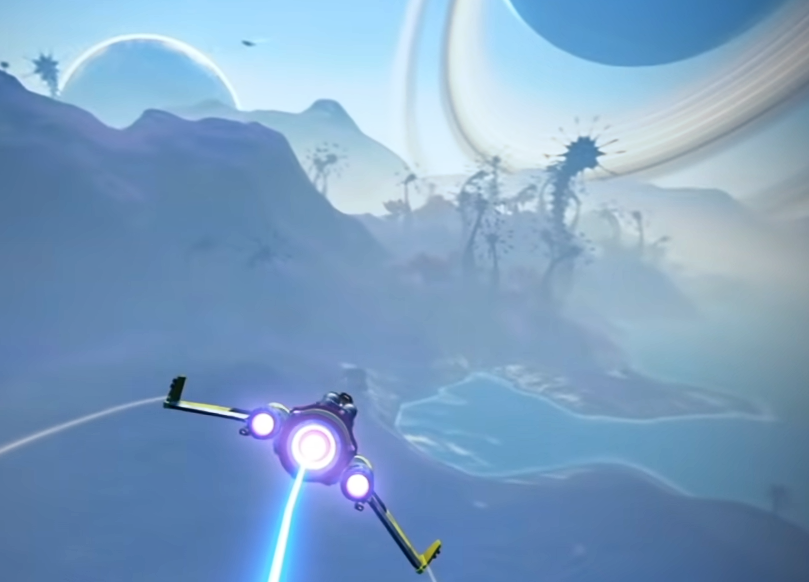
\includegraphics[height=0.55\textwidth]{image/nomanssky.png}
    
    \smallskip
    
    Részlet a \textit{No Man's Sky Origins} játékból (hivatalos trailer)
\end{frame}

\section{Egy új megoldás körvonalai: HoloDB}
\def\sectionshorttitle{HoloDB}

\begin{frame}
    \slidetitle{\sectionshorttitle}{Elvárások egy új megoldással szemben}
    
    \begin{itemize}
        \setlength\itemsep{0.5em}
        \pause \item relációs adatmodellre épül
        \pause \item deklaratív, finomhangolható, könnyen bővíthető
        \pause \item nem szükséges forrásadatbázis, de mintaként használható
        \pause \item nincs preparálási folyamat, szinte azonnal elindul
        \pause \item óriás adatmennyiséget is képes szimulálni, szinte tárhelyigény nélkül
        \pause \item az adatokat csak elérésükkor, on-the-fly számítja
        \pause \item indexeket szolgáltat, ahol egyébként is elvárható lenne
        \pause \item a runtime teljesítmény kielégítő
        \pause \item determinisztikus, konzisztens, skálázható
        \pause \item opcionálisan írható
    \end{itemize}
\end{frame}

\begin{frame}
    \slidetitle{\sectionshorttitle}{Mit tapasztal a felhasználó?}
    
    \begin{itemize}
        \setlength\itemsep{1em}
        \item egyetlen átlátható, deklaratív konfigurációs fájlban minden megadható \pause
        \item nincs adatgenerálás, anonimizálás vagy egyéb preparálási folyamat \pause
        \item az adatbázis kis memóriaigénnyel fut \pause
        \item az adatbázis úgy viselkedik, mint egy valós relációs adatbázis \pause
        \item a lekérdezések elfogadható idő alatt lefutnak
    \end{itemize}
\end{frame}

\section{A HoloDB architektúrája}
\def\sectionshorttitle{Architektúra}

\begin{frame}
    \slidetitle{\sectionshorttitle}{Alapvető adattípus: LargeInteger}
    
    \begin{minipage}[t]{0.6\textwidth}
        \centering
        
        \vspace{0.5em}
        
        \begin{itemize}
            \setlength\itemsep{0.5em}
            \pause \item kis és óriás egészekkel is működik
            \pause \item a konverzió automatikus és egyértelmű
            \pause \item kis számokon gyors (\texttt{long} aritmetika)
            \pause \item memóriaigénye minimális
            \pause \item duplikálja a \texttt{BigInteger} metódusait
            \pause \item további hasznos metódusokkal bővíti
            \pause \item nincsenek függőségei
        \end{itemize}
    \end{minipage}%
    \begin{minipage}[t]{0.4\textwidth}
        \centering \pause
        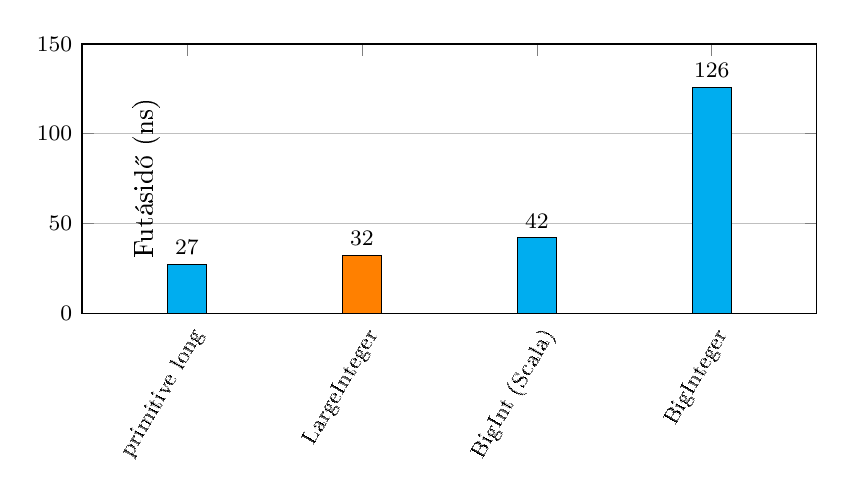
\begin{tikzpicture}[font=\footnotesize]
            \begin{axis}[
                    symbolic x coords={primitive long,,LargeInteger,,BigInt (Scala),,BigInteger},
                    xticklabel style={rotate=60,anchor=north east},
                    xtick={primitive long,LargeInteger,BigInt (Scala),BigInteger},
                    ylabel={Futásidő (ns)},
                    y label style={at={(0.12,0.5)}},
                    width={0.9\textwidth},
                    height=5cm,
                    ymajorgrids,
                    ymin=0,
                    ymax=150,
                    bar width=0.5cm,
                    enlarge x limits=0.2,
                    nodes near coords,
                    nodes near coords align={vertical},
                ]
                \addplot[ybar,fill=cyan] coordinates { (primitive long,27) };
                \addplot[ybar,fill=orange] coordinates { (LargeInteger,32) };
                \addplot[ybar,fill=cyan] coordinates { (BigInt (Scala),42) };
                \addplot[ybar,fill=cyan] coordinates { (BigInteger,126) };
            \end{axis}
        \end{tikzpicture}
    \end{minipage}
    
    \begin{flushright}
        { \footnotesize Benchmark: kis számokon végzett sokféle művelet ~~~~~ }
    \end{flushright}
\end{frame}

\begin{frame}
    \slidetitle{\sectionshorttitle}{Alapvető interfész: TreeRandom}
    
   (TODO: * TreeRandom ábra)
\end{frame}

\begin{frame}
    \slidetitle{\sectionshorttitle}{Vázlatos architektúraábra}
    
    \centering
    
    \begin{overprint}
        \onslide<1>\centerline{\includegraphics[height=0.65\textwidth]{diagram/simplearch-0}}
        \onslide<2>\centerline{\includegraphics[height=0.65\textwidth]{diagram/simplearch-1}}
    \end{overprint}
\end{frame}

\begin{frame}
    \slidetitle{\sectionshorttitle}{Storage API}
    
    (TODO: Storage API)
\end{frame}

\begin{frame}
    \slidetitle{\sectionshorttitle}{Írhatósági réteg}
    
    \pause A \texttt{DiffTable} dekorátor:
    
    \begin{itemize}
        \pause \item csak olvassa az alárendelt táblaobjektumot
        \pause \item amíg nincs módosítás, átlátszóan működik
        \pause \item memóriában tárolja a módosításokat
        \pause \item szükség szerint kiegészíti a lekérést és összefésüli az eredménytáblát
    \end{itemize}
    
    \vspace{0.4cm}
    
    \pause Tranzakciókezelés:
    
    \begin{itemize}
        \pause \item kétféle tranzakciós stratégia: írási ablakok vagy MVCC
        \pause \item kétféle commit mód: \texttt{AUTOCOMMIT} vagy explicit lockolás
        \pause \item mindegyik változat ACID-kompatibilis
        \pause \item nagyon sok írási művelet esetén nem igazán hatékony
    \end{itemize}
\end{frame}

\section{A szűk keresztmetszet: értékkiosztások}
\def\sectionshorttitle{Értékkiosztások}

\begin{frame}
    \slidetitle{\sectionshorttitle}{Az értékkiosztások problémaköre}

    \begin{itemize}
        \setlength\itemsep{1em}
        \pause \item Oszloporientáltság
        \pause \item Adatelérés (random access)
        \pause \item Ha lehet, keresés és rendezés (reverse index)
        \pause \item $NULL$ értékek
        \pause \item Előfordulási gyakoriságok
        \pause \item Esetenként többoszlopos
    \end{itemize}
\end{frame}

\begin{frame}
    \slidetitle{\sectionshorttitle}{Főbb egyoszlopos értékkiosztási típusok}

    \pause Nem indexelt
    
    \begin{itemize}
        \pause \item Egyszerű/strukturált szöveg
        \pause \item Strukturált adat
        \pause \item Kép
        \pause \item Jelszó-hash
        \pause \item Random BLOB/CLOB
    \end{itemize}
    
    \pause Indexelt
    
    \begin{itemize}
        \pause \item Számláló (például numerikus kulcsokhoz)
        \pause \item Időbélyegek, adott eloszlással és zajjal
        \pause \item Full-text indexelt szövegek
        \pause \item Általános kétfázisú értékkiosztás
    \end{itemize}
    
\end{frame}

\begin{frame}
    \slidetitle{\sectionshorttitle}{Általános kétfázisú értékkiosztás}
    
    \centering
    
    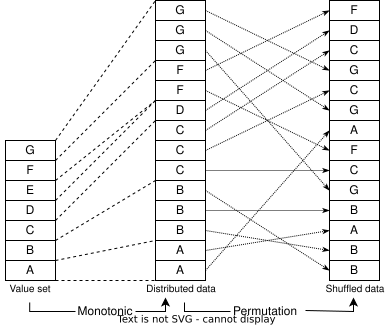
\includegraphics[height=0.5\textwidth]{diagram/distribution}
    
    Kétfázisú értékkiosztás alapelve: \par
    visszafejthető disztribúció és permutáció kompozíciója
\end{frame}

\begin{frame}
    \slidetitle{\sectionshorttitle}{Az értékkészlet interfész-tulajdonságai}
    
    \begin{itemize}
        \setlength\itemsep{1em}
        \pause \item Rendezett
        \pause \item Nincs ismétlődés (unique)
        \pause \item Lekérhető a lista hossza
        \pause \item Lekérhető az adott pozíción lévő érték (random access)
        \pause \item Lekérhető az adott érték pozíciója (reverse index) \par
              \pause ~ ~ ~ (ha az érték nem található, akkor a rendezés szerinti helye)
        \pause \item A lekérések gyorsan hajtódnak végre
    \end{itemize}
\end{frame}

\begin{frame}
    \slidetitle{\sectionshorttitle}{Tipikus kereshető értékkészletek}
    
    \begin{itemize}
        \setlength\itemsep{1em}
        \pause \item Szavak/kifejezések előre adott halmaza (például keresztnevek)
        \pause \item Numerikus sáv (például számok 1-től $n$-ig)
        \pause \item Reguláris kifejezésre illeszkedő szövegek
        \pause \item Külső forrásból betöltött indexelt értékkészlet
        \pause \item Összetett értékek (például teljes név, többdimenziós adat)
    \end{itemize}
\end{frame}

\begin{frame}
    \slidetitle{\sectionshorttitle}{Kétfázisú értékkiosztás: adatlekérés}
    
    \centering
    
    \begin{overprint}
        \onslide<1>\centerline{\includegraphics[height=0.45\textwidth]{diagram/getvalue-0}}
        \onslide<2>\centerline{\includegraphics[height=0.45\textwidth]{diagram/getvalue-1}}
        \onslide<3>\centerline{\includegraphics[height=0.45\textwidth]{diagram/getvalue-2}}
        \onslide<4>\centerline{\includegraphics[height=0.45\textwidth]{diagram/getvalue-3}}
        \onslide<5>\centerline{\includegraphics[height=0.45\textwidth]{diagram/getvalue-4}}
        \onslide<6->\centerline{\includegraphics[height=0.45\textwidth]{diagram/getvalue-5}}
    \end{overprint}
    
    \hspace{0.7cm}
    
    Adatlekérés a kétfázisú értékkiosztásból
\end{frame}

\begin{frame}
    \slidetitle{\sectionshorttitle}{Kétfázisú értékkiosztás: keresés}
    
    \centering
    
    \begin{overprint}
        \onslide<1>\centerline{\includegraphics[height=0.45\textwidth]{diagram/findvalue-0}}
        \onslide<2>\centerline{\includegraphics[height=0.45\textwidth]{diagram/findvalue-1}}
        \onslide<3>\centerline{\includegraphics[height=0.45\textwidth]{diagram/findvalue-2}}
        \onslide<4->\centerline{\includegraphics[height=0.45\textwidth]{diagram/findvalue-3}}
    \end{overprint}
    
    \vspace{0.5cm}
    
    Keresés a kétfázisú értékkiosztásban: \par
    A megfordíthatóság biztosítja a hatékony keresést
\end{frame}

\begin{frame}
    \slidetitle{\sectionshorttitle}{Kétfázisú értékkiosztás: nincs találat}
    
    \centering
    
    \begin{overprint}
        \onslide<1>\centerline{\includegraphics[height=0.45\textwidth]{diagram/findvalue-0}}
        \onslide<2>\centerline{\includegraphics[height=0.45\textwidth]{diagram/findvalue2-1}}
        \onslide<3>\centerline{\includegraphics[height=0.45\textwidth]{diagram/findvalue2-2}}
    \end{overprint}
    
    \vspace{0.5cm}
    
    Keresés a kétfázisú értékkiosztásban: \par
    A megfordíthatóság biztosítja a hatékony keresést
\end{frame}

\begin{frame}
    \slidetitle{\sectionshorttitle}{Kétfázisú értékkiosztás: nincs ilyen érték}
    
    \centering
    
    \begin{overprint}
        \onslide<1>\centerline{\includegraphics[height=0.45\textwidth]{diagram/findvalue-0}}
        \onslide<2>\centerline{\includegraphics[height=0.45\textwidth]{diagram/findvaluenone-1}}
        \onslide<3>\centerline{\includegraphics[height=0.45\textwidth]{diagram/findvaluenone-2}}
    \end{overprint}
    
    \vspace{0.5cm}
    
    Keresés a kétfázisú értékkiosztásban: \par
    A megfordíthatóság biztosítja a hatékony keresést
\end{frame}

\begin{frame}
    \slidetitle{\sectionshorttitle}{Kétfázisú értékkiosztás: értéksáv keresése}
    
    \centering
    
    \includegraphics[height=0.45\textwidth]{diagram/findvaluerange}
    
    \vspace{0.5cm}
    
    Keresés a kétfázisú értékkiosztásban: \par
    A megfordíthatóság biztosítja a hatékony keresést
\end{frame}

\section{Konfiguráció és bővítés}
\def\sectionshorttitle{Konfiguráció és bővítés}

\begin{frame}
    \slidetitle{\sectionshorttitle}{A konfiguráció jellemzői}
    
    \begin{itemize}
        \setlength\itemsep{0.5em}
        \pause \item konfigurációs fájllal leírható (alapértelmezetten YAML)
        \pause \item JPA entitásokra helyezett annotációkkal is definiálható
        \pause \item deklaratív, átlátható
        \pause \item a sémát és az adattartalmat integráltan írja le
        \pause \item a gyökér-\textt{seed} változtatásával mindent újrakeverhető
        \pause \item minden lényeges paraméter állítható
        \pause \item az igények nagy része lefedhető a beépített lehetőségekkel
        \pause \item ugyanakkor egyedi működés is beemelhető
        \pause \item megfelelő heurisztikákkal létező adatbázisról is mintázható
    \end{itemize}
\end{frame}

\begin{frame}[containsverbatim]
    \slidetitle{\sectionshorttitle}{Konfiguráció-példa}
    
    \centering
    \begin{minipage}[c]{0.47\textwidth}
        \begin{minted}[fontsize=\tiny,framesep=4pt,frame=single,framerule=1.5pt,rulecolor=\color{gray!30}]{yaml}
seed: 425364
schemas:
- name: shop
    tables:
    - name: customers
        size: 5
        columns:
        - name: id
            mode: COUNTER
        - name: firstname
            valuesBundle: forenames
        - name: lastname
            valuesBundle: surnames
        - name: birth
            valuesRange: [1950, 2000]
    - name: orders
        size: 12
        columns:
        - name: id
            mode: COUNTER
        - name: cid
            valuesForeignColumn:
                [customers, id]
        - name: product
            valuesBundle: fruits
        - name: quantity
            valuesRange: [1, 10]
        \end{minted}
        \pause
    \end{minipage}%
    \hspace*{\fill}
    \begin{minipage}[c]{0.35cm}
        {\Large $\Rightarrow$}
    \end{minipage}%
    \hspace*{\fill}
    \begin{minipage}[c]{0.45\textwidth}
        
        \centering
        
        \normalsize \texttt{customers}
        \vspace{0.1cm}
        
        \tiny
        \begin{tabular}{ |r|l|l|r| }
        \hline
           id & firstname & lastname & birth \\
        \hline
            1 & Howard & Anderson & 1968 \\
            2 & Rebecca & Ferguson & 1959 \\
            3 & Jeremy & Moore & 2000 \\
            4 & Julie & Ellis & 1951 \\
            5 & Kathleen & Cook & 1971 \\
        \hline
        \end{tabular}
        
        \vspace{0.5cm}
        
        \normalsize \texttt{orders}
        \vspace{0.1cm}
        
        \tiny
        \begin{tabular}{ |r|r|l|r| }
        \hline
            id & cid & ~~product & quantity \\
        \hline
            1 & 5 & date & 10 \\
            2 & 2 & orange & 1 \\
            3 & 2 & sloe & 2 \\
            4 & 3 & melon & 7 \\
            5 & 5 & guava & 9 \\
            6 & 3 & orange & 6 \\
            7 & 2 & plantain & 3 \\
            8 & 4 & pear & 7 \\
            9 & 4 & papaya & 9 \\
            10 & 5 & lime & 9 \\
            11 & 3 & sloe & 4 \\
            12 & 1 & strawberry & 1 \\
        \hline
        \end{tabular}
    \end{minipage}
\end{frame}

% FIXME: pause doesn't work in the previous slide, so we duplicate the frame
\begin{frame}[containsverbatim,noframenumbering]
    \slidetitle{\sectionshorttitle}{Konfiguráció-példa}
    
    \centering
    \begin{minipage}[c]{0.47\textwidth}
        \begin{minted}[fontsize=\tiny,framesep=4pt,frame=single,framerule=1.5pt,rulecolor=\color{gray!30}]{yaml}
seed: 425364
schemas:
- name: shop
    tables:
    - name: customers
        size: 5
        columns:
        - name: id
            mode: COUNTER
        - name: firstname
            valuesBundle: forenames
        - name: lastname
            valuesBundle: surnames
        - name: birth
            valuesRange: [1950, 2000]
    - name: orders
        size: 12
        columns:
        - name: id
            mode: COUNTER
        - name: cid
            valuesForeignColumn:
                [customers, id]
        - name: product
            valuesBundle: fruits
        - name: quantity
            valuesRange: [1, 10]
        \end{minted}
    \end{minipage}%
    \hspace*{\fill}
    \begin{minipage}[c]{0.35cm}
        {\Large $\Rightarrow$}
    \end{minipage}%
    \hspace*{\fill}
    \begin{minipage}[c]{0.45\textwidth}
        
        \centering
        
        \normalsize \texttt{customers}
        \vspace{0.1cm}
        
        \tiny
        \begin{tabular}{ |r|l|l|r| }
        \hline
           id & firstname & lastname & birth \\
        \hline
            1 & Howard & Anderson & 1968 \\
            2 & Rebecca & Ferguson & 1959 \\
            3 & Jeremy & Moore & 2000 \\
            4 & Julie & Ellis & 1951 \\
            5 & Kathleen & Cook & 1971 \\
        \hline
        \end{tabular}
        
        \vspace{0.5cm}
        
        \normalsize \texttt{orders}
        \vspace{0.1cm}
        
        \tiny
        \begin{tabular}{ |r|r|l|r| }
        \hline
            id & cid & ~~product & quantity \\
        \hline
            1 & 5 & date & 10 \\
            2 & 2 & orange & 1 \\
            3 & 2 & sloe & 2 \\
            4 & 3 & melon & 7 \\
            5 & 5 & guava & 9 \\
            6 & 3 & orange & 6 \\
            7 & 2 & plantain & 3 \\
            8 & 4 & pear & 7 \\
            9 & 4 & papaya & 9 \\
            10 & 5 & lime & 9 \\
            11 & 3 & sloe & 4 \\
            12 & 1 & strawberry & 1 \\
        \hline
        \end{tabular}
    \end{minipage}
\end{frame}

\begin{frame}[containsverbatim]
    \slidetitle{\sectionshorttitle}{Egyedi működés hozzáadása}
    
    Egyedi értékkiosztás betöltése saját programkönyvtárból:
    
    \vspace{0.5em}
    
    \begin{minted}[fontsize=\small,framesep=4pt,frame=single,framerule=1.5pt,rulecolor=\color{gray!30}]{yaml}
- name: some_column
  sourceFactory: org.example.myorg.SomeCustomDataFactory
  sourceFactoryData:
      additionalParameter1: 10
      additionalParameter2: 'lorem ipsum'
    \end{minted}
    
    \vspace{1em}
    
    Egyedi értékkészlet betöltése fájlból:
    
    \vspace{0.5em}
    
    \begin{minted}[fontsize=\small,framesep=4pt,frame=single,framerule=1.5pt,rulecolor=\color{gray!30}]{yaml}
- name: some_column
  valuesResource: custom-data.txt
    \end{minted}
    
\end{frame}

\begin{frame}
    \slidetitle{\sectionshorttitle}{Bővítés: valós postai címek használata}
    
    Cím hierarchiája:
    
    \begin{center}
        településnév ~ $\rightarrow$ ~
        kerület ~ $\rightarrow$ ~
        közterület neve ~ $\rightarrow$ ~
        közterület jellege ~ $\rightarrow$ ~
        házszám ~ $\rightarrow$ ~
        egyéb
    \end{center}
    
    \begin{itemize}
        \setlength\itemsep{0.5em}
        \pause \item az összes létező címet leképezzük a táblára (pl. kétfázisú értékiosztással)
        
    \end{itemize}

    (TODO: Bővítés: valós címek használata)
\end{frame}

\begin{frame}
    \slidetitle{\sectionshorttitle}{Bővítés: on-demand schema}
    
    \begin{itemize}
        \setlength\itemsep{1em}
        \pause \item Nincs előre megadott séma
        \pause \item Ha egy lekérés új táblát/oszlopot tartalmaz, on-demand létrehozzuk
        \pause \item Új táblából történő wildcardos lekérdezésnél alapértelmezett oszlop
        \pause \item Táblaméret, oszloptípus, idegen kulcs megállapítása heurisztikákkal
        \pause \item A \texttt{seed} lehet beégetett vagy az első lekérés függvénye
        \pause \item Írható adatbázis esetén nehéz megvalósítani
    \end{itemize}
\end{frame}

\section{Eredmények}
\def\sectionshorttitle{Eredmények}

\begin{frame}
    \slidetitle{\sectionshorttitle}{Tárhelyigény}
    
    \begin{minipage}[b]{0.34\textwidth}
        \centering
        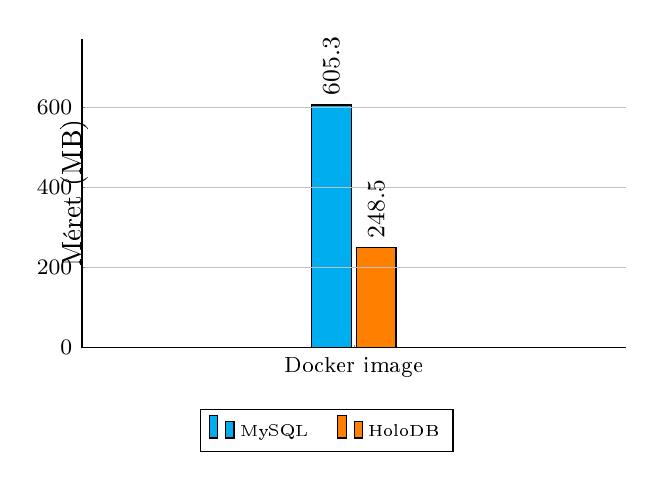
\begin{tikzpicture}
            \begin{axis}[
                    symbolic x coords={Docker image},
                    ybar,
                    axis on top,
                    width={0.7\textwidth},
                    height=5.5cm,
                    bar width=0.5cm,
                    ymajorgrids,
                    tick align=inside,
                    enlarge y limits={value=.1,upper},
                    enlarge x limits=0.15,
                    ymin=0,
                    ymax=700,
                    point meta=rawy,
                    every node near coord/.append style={
                        anchor=west,
                        rotate=90,
                        font=\small
                    },
                    axis x line*=bottom,
                    axis y line*=left,
                    tickwidth=1pt,
                    legend style={
                        at={(0.45,-0.2)},
                        anchor=north,
                        legend columns=-1,
                        /tikz/every even column/.append style={column sep=0.3cm}
                    },
                    ylabel={Méret (MB)},
                    y label style={at={(0.03,0.5)}},
                    xtick=data,
                    nodes near coords={
                        \pgfmathprintnumber{\pgfplotspointmeta}
                    },
                    nodes near coords style={
                        /pgf/number format/.cd,
                        /pgf/number format/fixed,
                        precision=3
                    }
                ]
                \addplot[fill=cyan] % MySQL
                    coordinates { (Docker image,605.3) };
                \addplot[fill=orange] % HoloDB
                    coordinates { (Docker image,248.5) };
                \legend{MySQL,HoloDB}
            \end{axis}
        \end{tikzpicture}
    \end{minipage}%
    \begin{minipage}[b]{0.25\textwidth}
        \centering
        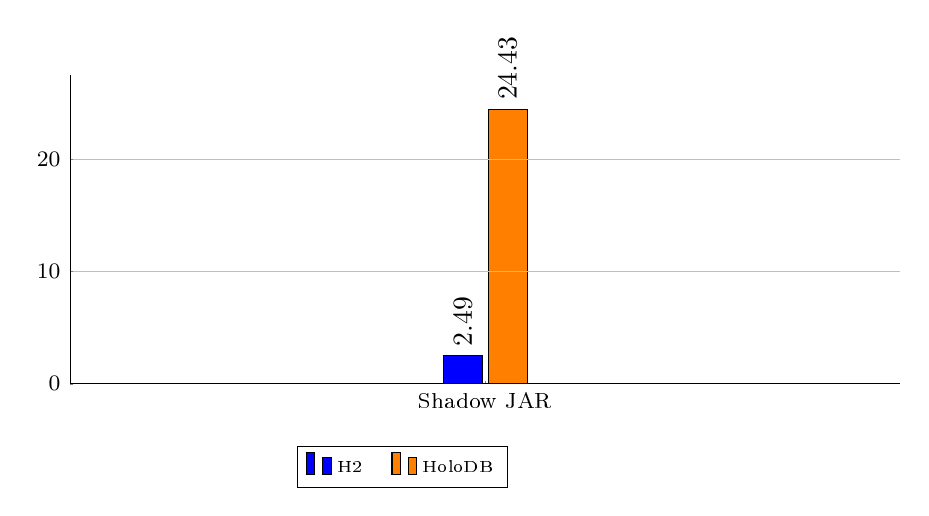
\begin{tikzpicture}
            \begin{axis}[
                    symbolic x coords={Shadow JAR},
                    ybar,
                    axis on top,
                    width={\textwidth},
                    height=5.5cm,
                    bar width=0.5cm,
                    ymajorgrids,
                    tick align=inside,
                    enlarge y limits={value=.1,upper},
                    enlarge x limits=0.15,
                    ymin=0,
                    ymax=25,
                    point meta=rawy,
                    every node near coord/.append style={
                        anchor=west,
                        rotate=90,
                        font=\smal
                    },
                    axis x line*=bottom,
                    axis y line*=left,
                    tickwidth=1pt,
                    legend style={
                        at={(0.4,-0.2)},
                        anchor=north,
                        legend columns=-1,
                        /tikz/every even column/.append style={column sep=0.3cm}
                    },
                    xtick=data,
                    nodes near coords={
                        \pgfmathprintnumber{\pgfplotspointmeta}
                    },
                    nodes near coords style={
                        /pgf/number format/.cd,
                        /pgf/number format/fixed,
                        precision=3
                    }
                ]
                \addplot[fill=blue] % H2
                    coordinates { (Shadow JAR,2.49) };
                \addplot[fill=orange] % HoloDB
                    coordinates { (Shadow JAR,24.43) };
                \legend{H2,HoloDB}
            \end{axis}
        \end{tikzpicture}
    \end{minipage}%
    \begin{minipage}[b]{0.3\textwidth}
        \centering
        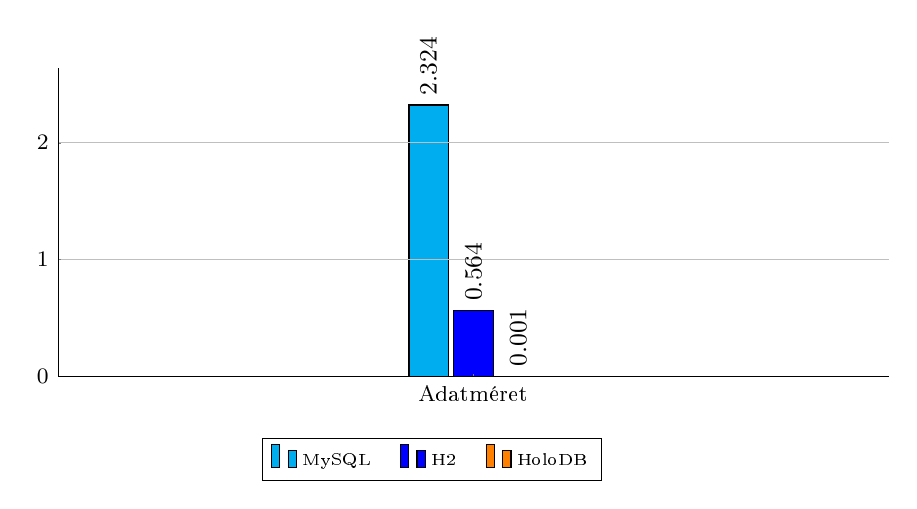
\begin{tikzpicture}
            \begin{axis}[
                    symbolic x coords={Adatméret},
                    ybar,
                    axis on top,
                    width={\textwidth},
                    height=5.5cm,
                    bar width=0.5cm,
                    ymajorgrids,
                    tick align=inside,
                    enlarge y limits={value=.1,upper},
                    enlarge x limits=0.15,
                    ymin=0,
                    ymax=2.4,
                    point meta=rawy,
                    every node near coord/.append style={
                        anchor=west,
                        rotate=90,
                        font=\small
                    },
                    axis x line*=bottom,
                    axis y line*=left,
                    tickwidth=1pt,
                    legend style={
                        at={(0.45,-0.2)},
                        anchor=north,
                        legend columns=-1,
                        /tikz/every even column/.append style={column sep=0.3cm}
                    },
                    xtick=data,
                    nodes near coords={
                        \pgfmathprintnumber{\pgfplotspointmeta}
                    },
                    nodes near coords style={
                        /pgf/number format/.cd,
                        /pgf/number format/fixed,
                        precision=3
                    }
                ]
                \addplot[fill=cyan] % MySQL
                    coordinates { (Adatméret,2.324) };
                \addplot[fill=blue] % H2
                    coordinates { (Adatméret,0.564) };
                \addplot[fill=orange] % HoloDB
                    coordinates { (Adatméret,0.001) };
                \legend{MySQL,H2,HoloDB}
            \end{axis}
        \end{tikzpicture}
    \end{minipage}
\end{frame}

\begin{frame}
    \slidetitle{\sectionshorttitle}{Integrált teszt futási ideje (Micronaut$,$ REST)}
    
    \centering
    
    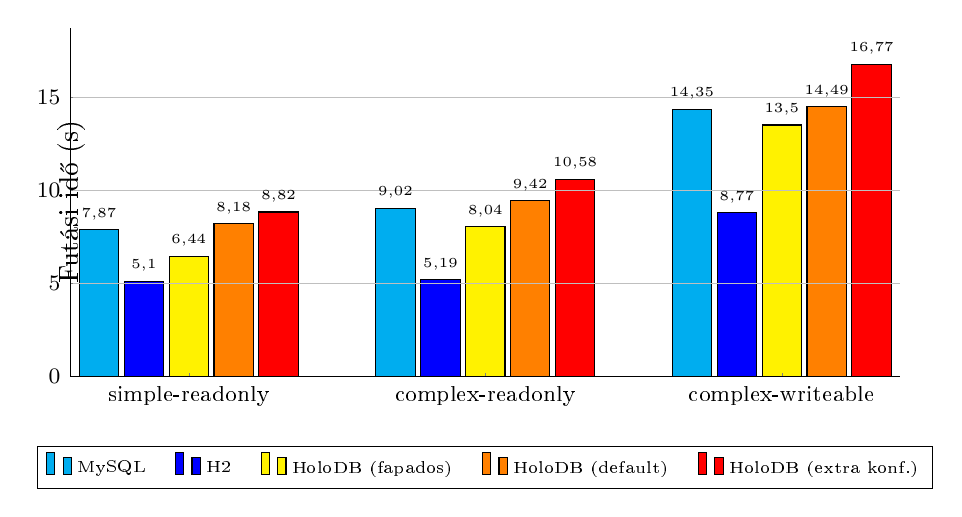
\begin{tikzpicture}[font=\tiny]
        \begin{axis}[
                symbolic x coords={simple-readonly,complex-readonly,complex-writeable},
                ybar,
                axis on top,
                width={\textwidth},
                height=6cm,
                bar width=0.5cm,
                ymajorgrids,
                tick align=inside,
                enlarge y limits={value=.1,upper},
                enlarge x limits=0.2,
                ymin=0,
                ymax=17,
                /pgf/number format/.cd,
                use comma,
                1000 sep={~},
                axis x line*=bottom,
                axis y line*=left,
                tickwidth=1pt,
                legend style={
                    at={(0.5,-0.2)},
                    anchor=north,
                    legend columns=-1,
                    font = {\fontsize{6 pt}{10 pt}\selectfont},
                    /tikz/every even column/.append style={column sep=0.3cm}
                },
                ylabel={Futási idő (s)},
                y label style={at={(0.03,0.5)}},
                xtick=data,
                nodes near coords={
                    \pgfmathprintnumber{\pgfplotspointmeta}
                }
            ]
            \addplot[fill=cyan] % MySQL
                coordinates {
                    (simple-readonly,7.870093628)
                    (complex-readonly,9.0179515675)
                    (complex-writeable,14.3489598653)
                };
            \addplot[fill=blue] % H2
                coordinates {
                    (simple-readonly,5.103988787)
                    (complex-readonly,5.1902669386)
                    (complex-writeable,8.7714582641)
                };
            \addplot[fill=yellow] % HoloDB (fapados)
                coordinates {
                    (simple-readonly,6.441775179)
                    (complex-readonly,8.0399578991)
                    (complex-writeable,13.4957423082)
                };
            \addplot[fill=orange] % HoloDB (default)
                coordinates {
                    (simple-readonly,8.182373242)
                    (complex-readonly,9.4207860077)
                    (complex-writeable,14.4941282014)
                };
            \addplot[fill=red] % HoloDB (extra konf.)
                coordinates {
                    (simple-readonly,8.819935654)
                    (complex-readonly,10.5782986771)
                    (complex-writeable,16.7720866313)
                };
            \legend{MySQL,H2,HoloDB (fapados),HoloDB (default),HoloDB (extra konf.)}
        \end{axis}
    \end{tikzpicture}
\end{frame}

\begin{frame}
    \slidetitle{\sectionshorttitle}{Átlagos futási idők összehasonlítása (log.)}
    
    \centering
    
    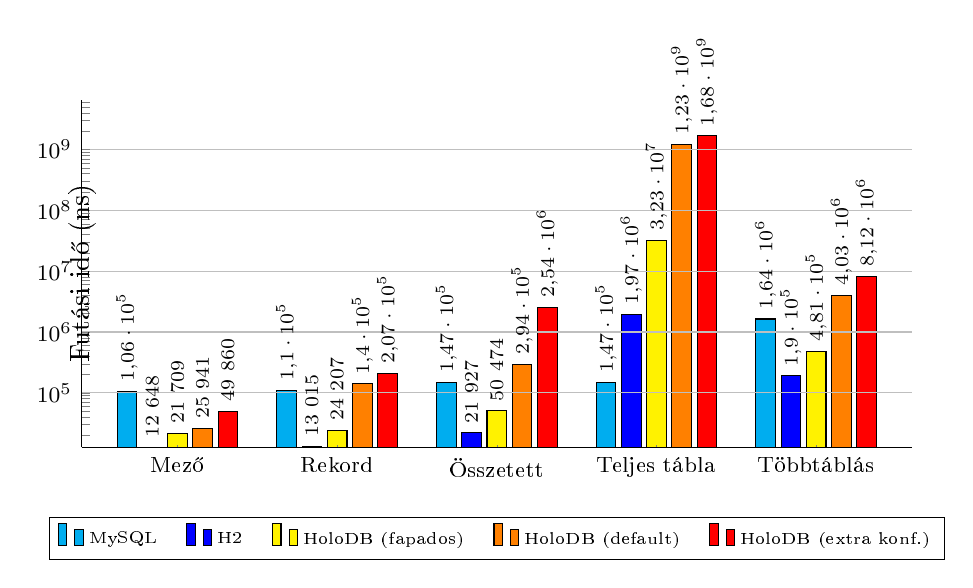
\begin{tikzpicture}[font=\scriptsize]
        \begin{axis}[
                title style={
                    at={(-0.1,1.15)},
                    anchor=north west
                },
                symbolic x coords={Mező,Rekord,Összetett,Teljes tábla,Többtáblás},
                ybar,
                axis on top,
                width={\textwidth},
                height=6cm,
                bar width=0.25cm,
                ymajorgrids,
                tick align=inside,
                enlarge y limits={value=.1,upper},
                enlarge x limits=0.15,
                ymin=0,
                ymax=2000000000,
                ymode=log,
                point meta=rawy,
                /pgf/number format/.cd,
                use comma,
                1000 sep={~},
                every node near coord/.append style={
                    anchor=west,
                    rotate=90
                },
                axis x line*=bottom,
                axis y line*=left,
                tickwidth=1pt,
                legend style={
                    at={(0.5,-0.2)},
                    anchor=north,
                    legend columns=-1,
                    font = {\fontsize{6 pt}{10 pt}\selectfont},
                    /tikz/every even column/.append style={column sep=0.3cm}
                },
                ylabel={Futási idő (ns)},
                y label style={at={(0.03,0.5)}},
                xtick=data,
                nodes near coords={
                    \pgfmathprintnumber{\pgfplotspointmeta}
                }
            ]
            \addplot[fill=cyan] % MySQL
                coordinates {
                    (Mező,106276)
                    (Rekord,109819) 
                    (Összetett,146710)
                    (Teljes tábla,146710)
                    (Többtáblás,1637889)
                };
            \addplot[fill=blue] % H2
                coordinates {
                    (Mező,12648)
                    (Rekord,13015) 
                    (Összetett,21927)
                    (Teljes tábla,1971234)
                    (Többtáblás,189958)
                };
            \addplot[fill=yellow] % HoloDB (fapados)
                coordinates {
                    (Mező,21709)
                    (Rekord,24207) 
                    (Összetett,50474)
                    (Teljes tábla,32271101)
                    (Többtáblás,481306)
                };
            \addplot[fill=orange] % HoloDB (default)
                coordinates {
                    (Mező,25941)
                    (Rekord,140232) 
                    (Összetett,293885)
                    (Teljes tábla,1228183178)
                    (Többtáblás,4030303)
                };
            \addplot[fill=red] % HoloDB (extra konf.
                coordinates {
                    (Mező,49860)
                    (Rekord,207383) 
                    (Összetett,2543441)
                    (Teljes tábla,1676796378)
                    (Többtáblás,8121736)
                };
            \legend{MySQL,H2,HoloDB (fapados),HoloDB (default),HoloDB (extra konf.)}
        \end{axis}
    \end{tikzpicture}
\end{frame}

\section{Összegzés}
\def\sectionshorttitle{Összegzés}

\begin{frame}
    \slidetitle{\sectionshorttitle}{Elvárások teljesítése}
    
    \begin{itemize}
        \setlength\itemsep{0.5em}
        \item[] \onslide<2->{\greencheck} relációs adatmodellre épül
        \item[] \onslide<3->{\greencheck} deklaratív, finomhangolható, könnyen bővíthető
        \item[] \onslide<4->{\greencheck} nem szükséges forrásadatbázis, de mintaként használható
        \item[] \onslide<5->{\greencheck} nincs preparálási folyamat, szinte azonnal elindul
        \item[] \onslide<6->{\greencheck} óriás adatmennyiséget is képes szimulálni, szinte tárhelyigény nélkül
        \item[] \onslide<7->{\greencheck} az adatokat csak elérésükkor, on-the-fly számítja
        \item[] \onslide<8->{\greencheck} a runtime teljesítmény kielégítő
        \item[] \onslide<9->{\greencheck} determinisztikus, konzisztens, skálázható
        \item[] \onslide<10->{\greencheck} opcionálisan írható
    \end{itemize}
\end{frame}

\begin{frame}
    \slidetitle{\sectionshorttitle}{További előnyök}
    
    \begin{itemize}
        \setlength\itemsep{1em}
        \pause \item könnyen verziókezelhető konfigurációs fájl
        \pause \item könnyű replikálhatóság (csak-olvasható adatbázis esetén)
        \pause \item teljesen izolált automatikus integrációs tesztelés adatbázissal
        \pause \item füsttesztek teljes értékű adatbázissal
        \pause \item írási rétegként létező adatbázis fölé is elhelyezhető
    \end{itemize}
\end{frame}

\begin{frame}
    \slidetitle{\sectionshorttitle}{TODO}
    
    (TODO: * Összefoglaláshoz még)
\end{frame}

\begin{frame}
    \slidetitle{\sectionshorttitle}{Miért nem terjedt még el hasonló megoldás?}

    \begin{itemize}
        \setlength\itemsep{1em}
        \pause \item \textbf{kontraintuitivitás}:
            előzetes feltevésemmel szemben úgy tűnik, nem olyan egyszerű átlátni a koncepciót,
            és megérteni hogy ``hol is vannak az adatok''
        \pause \item \textbf{megfelelő SQL plannerek eddigi hiánya}:
            az Apache Calcite például csak az utóbbi néhány évben vált népszerűvé,
            és inkább elsősorban adatintegrátorként
        \pause \item \textbf{bejáratott alternatívák}:
            az on-the-fly mockolás lehetősége,
            a NoSQL adatbázisok és felhőmegoldások fejlődése stb.
            sztenderdképző kerülőmegoldásokként elfedték a problémát
        \pause \item \textbf{érdekhiány}:
            nincs nyomás jelentősen más típusú termékkel való kísérletezésre,
            a nagy adatbázisvendorok érdeke elsősorban
            a tényleges adatbázisok kezelésére kínált megoldások fejlesztése
    \end{itemize}
\end{frame}

\begin{frame}
    \slidetitle{\sectionshorttitle}{Jövőbeli tervek}

    \begin{itemize}
        \setlength\itemsep{1em}
        \pause \item az alapvető működés optimalizálása
        \pause \item további kiegészítő funkciók, eszközök fejlesztése
        \pause \item dokumentáció és kommunikáció
        \pause \item megfelelő elnevezés megtalálása
            
            \vspace{0.5\baselineskip}
            
            \pause { \huge ~~~ } \faWifi ~~ \textit{holografikus adatbázis}
            
            \vspace{0.4\baselineskip}
            
            \pause { \huge ~~~ } ~\faGhost ~~ \textit{fantomadatbázis}
            
            \vspace{0.4\baselineskip}
            
            \pause { \huge ~~~ } ~\faEdit ~ \textit{deklaratív adatbázis}
    \end{itemize}
\end{frame}
        
\begin{frame}
    \vspace{1em}
    
    \centering
    
    { \Huge Köszönöm a figyelmet! }
    
    \vspace{3em}
    
    \begin{flushleft}
        \normalsize
        
        ~~~
        { \color{beamer@blendedblue} Projektlinkek: }
        
        \vspace{0.5em}
        
        \footnotesize
        
        \begin{itemize}
            \item HoloDB projekt: \par
                    \url{https://github.com/miniconnect/holodb}
            \item Használati példák: \par
                    \url{https://github.com/miniconnect/general-docs/tree/main/examples}
            \item Jelen TDK-pályamunka forrásrepója: \par
                    \url{https://github.com/davidsusu/holodb-tdk}
        \end{itemize}
    
        \vspace{1.5em}
        
        \normalsize
        
        ~~~
        { \color{beamer@blendedblue} E-mail: }
        \href{mailto:horvathdown@student.elte.hu}{horvathdown@student.elte.hu}
        \end{flushleft}
\end{frame}

\end{document}
